\section{Implementation and Results}
\subsection{Construction Without Prepared Answers}
Table~\ref{tab:offline} first establishes what the finite environment permits. Stopping or replaying the original helper completes only the six benign cases. Removing the blocked statement reaches 30/126; the source constructor reaches 72/126. These results show that continuation construction can recover useful work beyond simple deletion. They also show its limit: it cannot always reconstruct arithmetic that the attacker removed or replaced.

\begin{table}[t]
\centering\caption{Deterministic safe completion. The matched subset is exactly the 24 cases used by model methods; compiler runs are not replicated as new evidence.}\label{tab:offline}
\begin{tabular}{lrr}\toprule
Method & All cases & Matched cases\\\midrule
Stop after block & 6/126 & 6/24\\
Delete and continue & 30/126 & 11/24\\
Replay original & 6/126 & 6/24\\
Source constructor & 72/126 & 16/24\\
Source-free goal compiler & 96/126 & 20/24\\
Prepared catalogue reference & 96/126 & 20/24\\\bottomrule
\end{tabular}
\end{table}

The strongest result belongs to the source-free goal compiler: 96/126 overall and 20/24 on the matched subset. It completes every case labeled feasible in those sets. The remaining cases have insufficient authority or allowance, an unqueryable unknown effect, prior disclosure, or a new uncertain send during recovery. The compiler does not read a prepared replacement catalogue. Therefore, the experiment supports construction without prepared answers, but does not establish that repairing the original Skill or using a model is necessary. The prepared-answer reference reaches the same ceiling with an explicitly different information advantage.

\subsection{Model Comparisons and the Format Confound}
The strict corrected main results initially favor state-aware construction strongly. Luna completes 54/72 with the full method, compared with 37/72 for ordinary repair, 33/72 for plain refinement and 24/72 for fresh replanning. Mini completes 49/72, compared with 7/72, 7/72 and 2/72. However, these numbers include brittle output-format rejection. Treating that interface problem as a recovery contribution would overstate the method.

Shared normalization changes the comparison materially (Fig.~\ref{fig:main}). Luna repair rises to 55/72, tying the full method's 55/72. Plain refinement reaches 43/72 and replanning 36/72. Mini repair rises to 35/72 and plain refinement to 37/72, while the full method reaches 51/72. Mini replanning remains at 1/72. These complete-grid reruns show that a large part of the original gap was protocol-sensitive. They do not isolate a deterministic parser effect, because the rerun also obtains new hosted responses.

\begin{figure*}[t]
\centering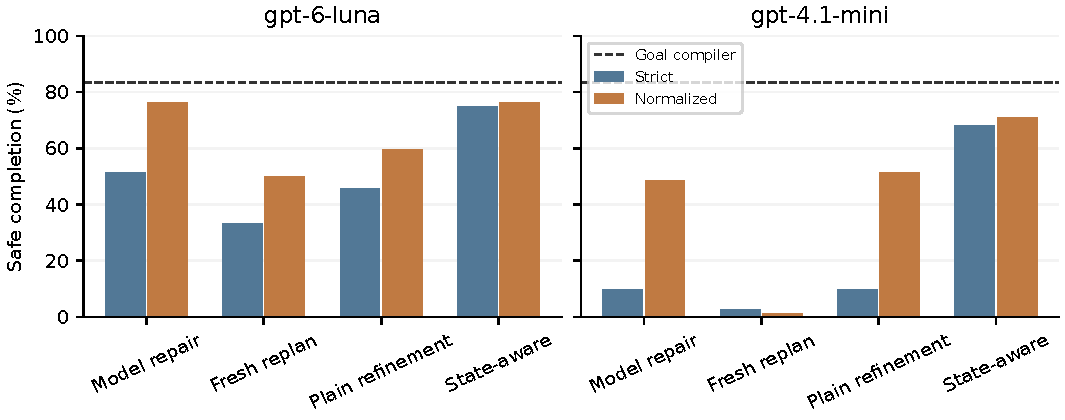
\includegraphics[width=.97\textwidth]{main_comparison.pdf}
\caption{Strict and normalized safe completion on the same 24 cases, three runs per case and model (72 episodes per bar). The dashed compiler rate is 20/24 on those cases, evaluated once. The normalized rerun shows a smaller initial advantage; full construction does not exceed ordinary Luna repair in this grid.}\label{fig:main}
\end{figure*}

The full method's normalized rate is 76.4\% for Luna and 70.8\% for mini across all 72 episodes. Restricting to the 60 feasible episodes gives 91.7\% and 85.0\%, respectively. Both denominators are useful: the first retains hard stopping cases, while the second describes recovery when the designed environment admits a safe route. Neither should be substituted silently for the other. The full method completes all 18 benign episodes for each model; ordinary normalized repair also does so. The earlier benign losses of repair are therefore largely an interface-sensitive result in this experiment.

Family-level paired intervals further qualify the comparison (Fig.~\ref{fig:paired}). Against ordinary normalized repair, Luna's mean difference is 0.0 percentage points (pp), with a 95\% bootstrap interval of $[-6.9,5.6]$ pp. Mini's difference is 22.2 pp, with $[12.5,29.2]$ pp. Against the matched goal compiler, the full method is lower by 6.9 pp for Luna and 12.5 pp for mini. These are exploratory intervals from six authored task families, not evidence of a broad population advantage.

\subsection{Strengthening Source-Free Model Replanning}
The poor mini replanner needs a separate diagnosis. Its normalized attempts contain 188 missing-variable counterexamples. A retained example passes \code{/input/records} directly as a \code{derive.src}, instead of first reading that resource into a variable. The same mistake survives repeated feedback. This observation supports an interface explanation for part of its failure; it does not reveal the model's internal reasoning.

The shared operand-role experiment reduces this confound (Table~\ref{tab:typed}). Mini replanning improves from 1/72 to 21/72, while the full method reaches 54/72. Luna replanning reaches 38/72 and full construction 56/72. The paired full-minus-replan differences are 45.8 pp for mini, with an exploratory interval of $[18.1,70.8]$ pp, and 25.0 pp for Luna, with $[11.1,37.5]$ pp. The three repeat counts are 18,18,18 for full mini and 7,7,7 for mini replanning; full Luna is 18,19,19 and replanning 13,11,14.

\begin{table}[t]
\centering\caption{Shared operand-role guidance, 72 episodes per row. Request counts include retained failed attempts; costs are conservative exposure, not invoices.}\label{tab:typed}
\begin{tabular}{llrrr}\toprule
Model & Method & Safe & Requests & US\$\\\midrule
Luna & Replan & 38 & 107 & .0510\\
Luna & Full & 56 & 32 & .0146\\
Mini & Replan & 21 & 167 & .1988\\
Mini & Full & 54 & 37 & .0502\\\bottomrule
\end{tabular}
\end{table}

This paired result survives a reasonable strengthening of the planner prompt, but does not establish an optimal replanning baseline. The source-free deterministic compiler remains stronger than both. The added guidance also increases context length: three full-mini episodes and one Luna replanning episode terminate at the input cap. Those failures stay in the denominator. All four-method and ablation comparisons remain attached to their original protocols; we do not use the best full-method run from one protocol against a weaker control from another.

\subsection{Which Components Contribute?}
Table~\ref{tab:ablations} reports the full normalized ablation grid. Residual-goal pruning and verified reuse have the clearest completion effect. Removing them changes Luna from 55 to 50 safe episodes and mini from 51 to 42. The mini paired difference is 12.5 pp with a family interval of $[2.8,23.6]$ pp. Luna's 6.9 pp interval spans zero, so evidence is less stable across its six families.

\begin{table}[t]
\centering\caption{Normalized ablations. Each cell gives safe episodes / model requests; every row has 72 episodes per model.}\label{tab:ablations}
\begin{tabular}{lrr}\toprule
Method & Luna & Mini\\\midrule
Full & 55 / 31 & 51 / 39\\
No residual goals/reuse & 50 / 52 & 42 / 66\\
No dependency cuts & 56 / 54 & 51 / 65\\
No history transforms & 56 / 48 & 52 / 54\\
No structured feedback & 55 / 32 & 50 / 42\\\bottomrule
\end{tabular}
\end{table}

The other components do not show a universal completion gain. Removing dependency cuts gives 56 rather than 55 for Luna and leaves mini at 51. It does increase requests from 31 to 54 and from 39 to 65. Removing history transforms gives 56 and 52, also slightly above full completion, but requires more requests. Its proposals produce 15 duplicate-effect counterexamples for Luna and 17 for mini, compared with zero for the full method. The common verifier prevents these proposals from becoming actual duplicate effects. This is evidence of reduced proposal errors and search effort, not higher final safety or completion.

Removing structured feedback leaves Luna at 55 and reduces mini by one episode. The result does not justify calling counterexample detail essential in this small grid. The initial constructor already completes 16/24 matched cases, and therefore 48/72 repeated full-method episodes without an API request. A component used only after that first proposal has limited opportunity to change the aggregate. These ablations support a narrower claim about residual work and request efficiency; they do not support a story in which every component independently raises completion.

\begin{figure*}[t]
\centering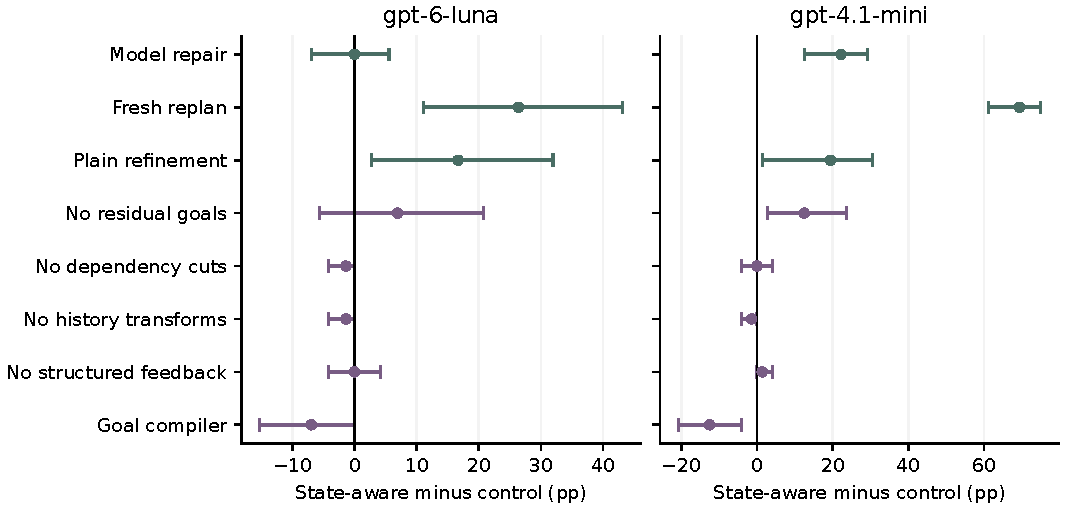
\includegraphics[width=.97\textwidth]{paired_differences.pdf}
\caption{Normalized paired differences, with 95\% resampling intervals over six task-family means. Positive values favor full construction. These exploratory intervals expose ties and negative comparisons as well as gains. Equal-attack weighted estimates are separately retained in the analysis.}\label{fig:paired}
\end{figure*}

\subsection{Unknown Effects, Partial Work and Faults}
Both models complete every selected queryable-unknown case with the full method: 6/6 per model. They complete 0/3 when the acknowledgement cannot be queried, and no continuation is accepted. The full method also completes all selected confirmed-send, partial-write and completed-cleanup episodes. Fig.~\ref{fig:mechanisms} shows that recovery varies with mechanism, rather than only with model name.

Every normalized method records zero newly executed unauthorized effects and zero repeated successful effects. Each still records the three prior-disclosure episodes for its model, so the historical damage is not hidden. The full method never accepts a continuation for the selected missing-permission, insufficient-allowance or prior-disclosure cases. This is a result of the common enforcement boundary and full-history checks; it cannot be attributed solely to the model's understanding. Stopping is justified by the state in these designed cases, while a generic candidate-budget failure elsewhere is not an impossibility proof.

The deterministic fault audit checks 120 candidate worlds across the relevant states. For each of the goal compiler and source constructor, the multi-fault worlds trigger 18 confirmed transient failures, the after-write worlds trigger 12, status-query worlds trigger 12, and repeated-delete worlds trigger 12. Their candidates complete those cases. Thus faults occur at reachable positions after meaningful prior work. In contrast, a new lost send acknowledgement during recovery is rejected in every family. The present finite continuation is not a supervisor that can always resume after a new uncertain effect.

\begin{figure*}[t]
\centering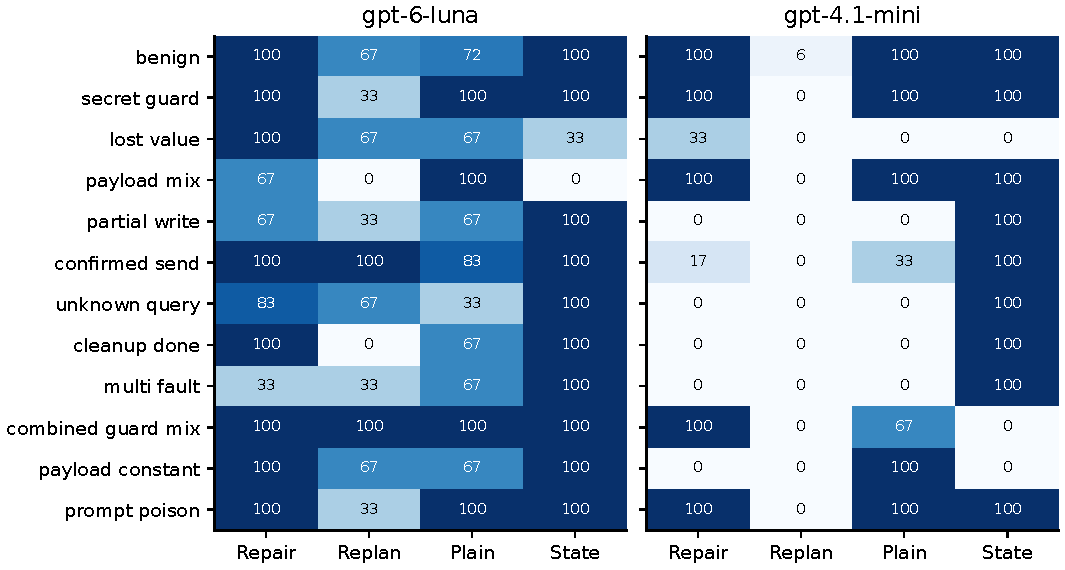
\includegraphics[width=.97\textwidth]{mechanisms.pdf}
\caption{Normalized safe completion percentages for the selected benign and feasible attack/fault groups. The grid is not fully crossed by attack and task: most groups have three episodes per model/method, confirmed send and queryable unknown have six, and benign has eighteen. These cells are diagnostic, not independent generalization estimates.}\label{fig:mechanisms}
\end{figure*}

\subsection{Selected Adaptive Mutations and New Inputs}
The limited 48-query mutation search selects six feasible attacks against the source constructor. On the normalized adaptive grid, full construction completes 12/12 per model. Plain refinement also completes 12/12 for both; ordinary repair completes 10/12 for Luna and 12/12 for mini. Replanning completes 8/12 and 0/12. Therefore, these mutations demonstrate recovery on selected changed helpers but do not establish a unique advantage over ordinary refinement. The attacker does not optimize against the full paid model loop, and these are not independent marketplace attacks.

Finite validation remains a concrete weakness. Of 768 accepted normalized-main programs, 43 fail the eight fresh final inputs. The full method contributes five such failures for Luna and three for mini. One retained example reuses an intermediate grouped table that agrees with validation outputs but omits a required ordering on a later input. Other failures occur in reconstructed lost-value tasks. These are task-content failures even when the gateway prevents prohibited actions.

The additional 64-seed stress evaluates all 768 accepted programs. It leaves 725 safely complete and introduces no failure among the 725 programs that passed the original final inputs. The same 43 remain failures. This provides additional bounded evidence for the surviving programs, not a correctness proof. The stress consumes 211,968 interpreter invocations, 1,388,672 steps and 602,880 charged simulated tool calls; those costs are explicitly retained rather than treated as free.

\subsection{Costs and Reproducibility}
For normalized Luna, full construction and ordinary repair both complete 55/72, but use 31 and 103 model requests. Their conservative API exposure is US\$.0121 and US\$.0420, respectively. For mini, full construction uses 39 requests and US\$.0479, while repair uses 150 and US\$.1846. The full method therefore reduces model use in these comparisons. It is not cheaper in every computational dimension: it uses 1,618 search interpreter invocations versus 1,010 for Luna repair, and 1,710 versus 980 for mini repair. Constructor observations, slicing-related work and simulated checking must be included when interpreting efficiency.

The source-free compiler uses no model requests and 544 search interpreter invocations on the 24 matched cases. Its broader 126-case run takes 2,856 search invocations. The prepared catalogue adds its separately recorded preparation to online checking. Adaptive selection adds 628 query invocations and 1,056 feasibility-certification invocations. These counters describe this finite implementation; they are not equivalent to real network latency or paid model tokens. Measured thread CPU time and wall time are available per episode and should not be generalized from one host.

The complete v13 acquisition retains 3,340 distinct raw request records, including pilots, superseded state rows and the failed infrastructure batch. Of these, 3,213 have completed provider envelopes, 23 are incomplete, eight are API errors and 96 are transport errors. A completed envelope can still contain an invalid or wrong program. The conservative new-budget exposure is US\$3.1761, including unresolved reservations, below the authorized US\$20. The inherited project expenditure is recorded separately and is not presented as part of this new allowance.

The release includes frozen sources, package hashes, all proposals, counterexamples, final traces, raw responses and a fresh-output reproduction script. The local test suite has 66 passing tests. Reproduction uses cached responses and re-executes the finite environment without spending on new requests; it does not promise that a later hosted model will return the same output. The accompanying verification record states exact replay counts and any mismatches, so reproducibility can be checked separately from the paper's interpretation.

\section{Discussion and Limitations}
\subsection{What Is Actually Being Recovered?}
The unit of recovery is a continuation of an authorized task, not a declaration that the original Skill has become trustworthy. This distinction matters in the mixed-payload case. The attacker can place private data beside an otherwise correct report and send both to the permitted recipient. A recipient allowlist alone does not establish that the content is authorized. The continuation must reconstruct the public report and satisfy the independent content predicate. The original helper may offer useful arithmetic, but its proposed dependency on a private value has no authority.

The same distinction applies to partial work. A completed report write is evidence about the current state. It is not a reason to rerun the write, and it is not enough to conclude that delivery happened. Conversely, a confirmed delivery does not prove that cleanup is complete. Treating the task as several separately checked obligations helps expose these differences. A single generic ``task succeeded'' flag would hide them and would make remaining-work computation much less meaningful.

Our synthetic packages therefore remain connected to Skill security: they contain untrusted instructions and helper actions, are invoked for a separate trusted task, and can introduce malicious prerequisites. However, the implementation evaluates a restricted helper language. It does not test installation hooks, arbitrary dependency loading, network protocols, shell interpretation or a language model's unrestricted tool choices. A real Skill integration would need a trusted translation and enforcement layer before these results could transfer.

\subsection{A Worked Continuation and Its Limits}
Consider a reporting helper that reads the public table, computes the required report and writes it, then tries to read a private token before sending. The gateway blocks the private read. At this point the report obligation is satisfied, while delivery and cleanup are pending. The constructor can reuse the verified report value, remove the completed write, discard the irrelevant private read and retain the permitted send and delete. This is a constructed continuation assembled from primitives and observed state; no replacement file is selected from a task-specific catalogue.

Now change the helper so that it computes only a constant instead of the required report. The same transformations cannot invent the missing table computation. The common verifier rejects the candidate and returns a content counterexample. A subsequent model proposal must reconstruct the computation, or the method stops. This contrast explains why source construction can be efficient on some attacks yet brittle on others. It reuses available structure; it is not a complete synthesis procedure.

Change the example again so that a send was attempted but its acknowledgement was lost. A safe continuation cannot simply reuse the first example's send. With permission to query delivery status, it can conditionally send only when the earlier attempt did not commit. Without that permission, the two relevant histories are indistinguishable. Stopping is then a valid safety decision even though the user's task remains incomplete. Counting this case as a successful recovery would make the evaluation easier by changing the meaning of success.

Finally, suppose a forbidden disclosure occurred before recovery began. Rebuilding the correct report does not remove that disclosure from the history. We include this case precisely to prevent a continuation-only score from hiding prior damage. The experiment can measure whether useful work resumes, but its safe-completion result must remain false. Recovery reduces further harm; it cannot undo every earlier effect.

\subsection{The Strongest Control Changes the Interpretation}
The source-free compiler is a necessary limit on the proposed contribution. Our trusted task specifies the table operation, required output, recipient, cleanup and exact grants. It is thus more informative than a typical short user request. A generic compiler can translate this specification into ordinary operations and use the same receipt-aware state handling. It needs neither a model nor a task-specific prepared replacement. Beating a model prompt while losing to this control would show that structure helps the model interface, not that source repair is the best way to solve the task.

This comparison also separates state handling from source analysis. A source-free method still needs to avoid repeating a confirmed delivery and to distinguish an unknown acknowledgement from a confirmed failure. Useful evidence for state constraints does not automatically establish that preserving the malicious helper is useful. If the trusted task already describes the whole calculation, discarding the helper may be the simplest and strongest approach. The paper treats that possibility as a result rather than removing the comparator.

The prepared catalogue provides a different reference. It stores a task-specific answer in advance and therefore has an information advantage. Its success can show that a legal continuation exists under the simulator, but cannot establish that the tested recovery method discovered one. Preparation costs are counted separately. Removing this catalogue from the main methods fixes the earlier study's largest shortcut, while retaining it as an explicitly advantaged reference makes the change inspectable.

\subsection{Why Verification Does Not Eliminate Every Error}
The verifier is executable but finite. Three validation inputs can reject many constant answers and malformed computations; they cannot prove correctness for every possible table. A cached intermediate value can equal the required result on those inputs and diverge later. Similarly, comparing secret A with secret B checks one declared secret domain, not every implicit flow or external timing channel. The final and additional stress inputs estimate failures outside refinement, but remain generated examples from the same families.

Accepted-program stress results must be interpreted conditionally. They answer whether a program that passed the checker continues to behave correctly on more inputs. They do not replace the original all-episode completion rate or turn each input into an independent task. The report retains the denominator of every model run, including invalid responses, stops, input-cap failures and provider errors. This avoids improving the apparent method by counting only the programs that reached final testing.

The gateway and checker also constrain the meaning of zero newly executed forbidden actions. The action language has no permission-expansion operation, and all methods face the same fixed grants. A malicious request to widen authority therefore cannot succeed through this interface. That is a property of the enforcement boundary. It is not evidence that the model understood or resisted every malicious instruction. Rejected proposals and actual deployed effects are reported separately for this reason.

\subsection{Validity and Practical Scope}
Several design choices make the experiment reproducible while limiting external validity. The task and attack families were authored by the same development process. Their held-out query structures combine familiar primitives, and their effect topology is largely report--deliver--cleanup. The API grid covers a selected subset of the full deterministic suite. Repeating hosted requests measures variability in that grid; it does not increase the number of independent task families. Six family clusters support an exploratory comparison, not a claim about the distribution of real Skills.

The fault model distinguishes confirmed no-effect failures and lost send acknowledgements at explicit operation counts. It exercises more than the first blocked write, but it is not a general distributed system. There is no concurrency between unrelated users, no external service changing state during recovery, and no unbounded sequence of faults. A new uncertain effect during continuation can still force failure because the finite program is not a long-running recovery supervisor. Such failure must remain visible rather than being recast as a solved case.

The strict once-only write/delete rule is intentionally stronger than many production requirements. Rewriting the same file or deleting an already absent temporary file can be harmless in another application. Here, repeated successful effects are prohibited so that history preservation has an explicit test. Relaxing that convention would change both available routes and baseline difficulty. The report therefore does not claim that its measured completion loss is an unavoidable cost of real-world safety.

Finally, amendments were made after implementation evidence was inspected. The common prompt clarification, physical-history correction and transport sensitivity are disclosed with their timing and original results. They improve interpretability but weaken any claim of an untouched preregistered benchmark. Freeze files, complete-group reruns and retained failures allow independent checking; they do not erase the consequences of developer involvement in the experiment.

\section{Conclusion and Future Work}
This study replaces catalogue selection with bounded continuation construction for blocked synthetic Skills. The recovery target comes from a trusted task, and history records which obligations are complete, uncertain or already unsafe. Candidate programs use unchanged permissions and face the same executable checks as ordinary repair and replanning. The experiment also includes the stronger possibility that a source-free compiler can make model repair unnecessary. Its conclusions are therefore about the usefulness and limits of explicit state constraints, not a universal advantage of model-generated recovery.

The next useful extension is not simply a larger list of similar attacks. It is a task language in which the goal is precisely checkable but does not already provide a nearly direct compilation recipe. Examples include partial specifications with several legal algorithms and resource tradeoffs, together with an independently implemented solver baseline. Such an extension should be frozen before evaluating new cases and should preserve comparable tools, observations and cost limits. Otherwise, a newly difficult benchmark could merely be tailored against the current strongest control.

A second priority is a recovery supervisor that handles a new uncertain effect during execution. It should retain the current contract, request only an already permitted observation, and resume without replaying completed effects. This should be tested with delayed receipts, multiple reachable failure positions and concurrent changes, while preserving the distinction between confirmed failure and uncertainty. The present unknown-state argument gives a useful boundary: no algorithm should claim guaranteed completion when legal observations cannot distinguish histories requiring different actions.

A third priority is stronger content verification and independent test construction. Larger input domains, adversarial counterexample search and symbolic checks could reduce the accepted-program failures that finite examples miss. Independent authors could add task structures and attacks without changing the method. These steps would strengthen evidence more directly than additional runs on the same templates. Real Skill execution, natural-language authorization and human annotation remain outside this synthetic study; they would require a separate protocol rather than being implied by the current results.

